\paragraph{Geographic Granularity.}
We analyze model performance across the geographic hierarchy by measuring whether responses correctly identify each level: the exact city (strict match), province/state, country, and world region. This reveals where in the hierarchy models' geographic knowledge breaks down.

\begin{figure}[htbp]
\centering
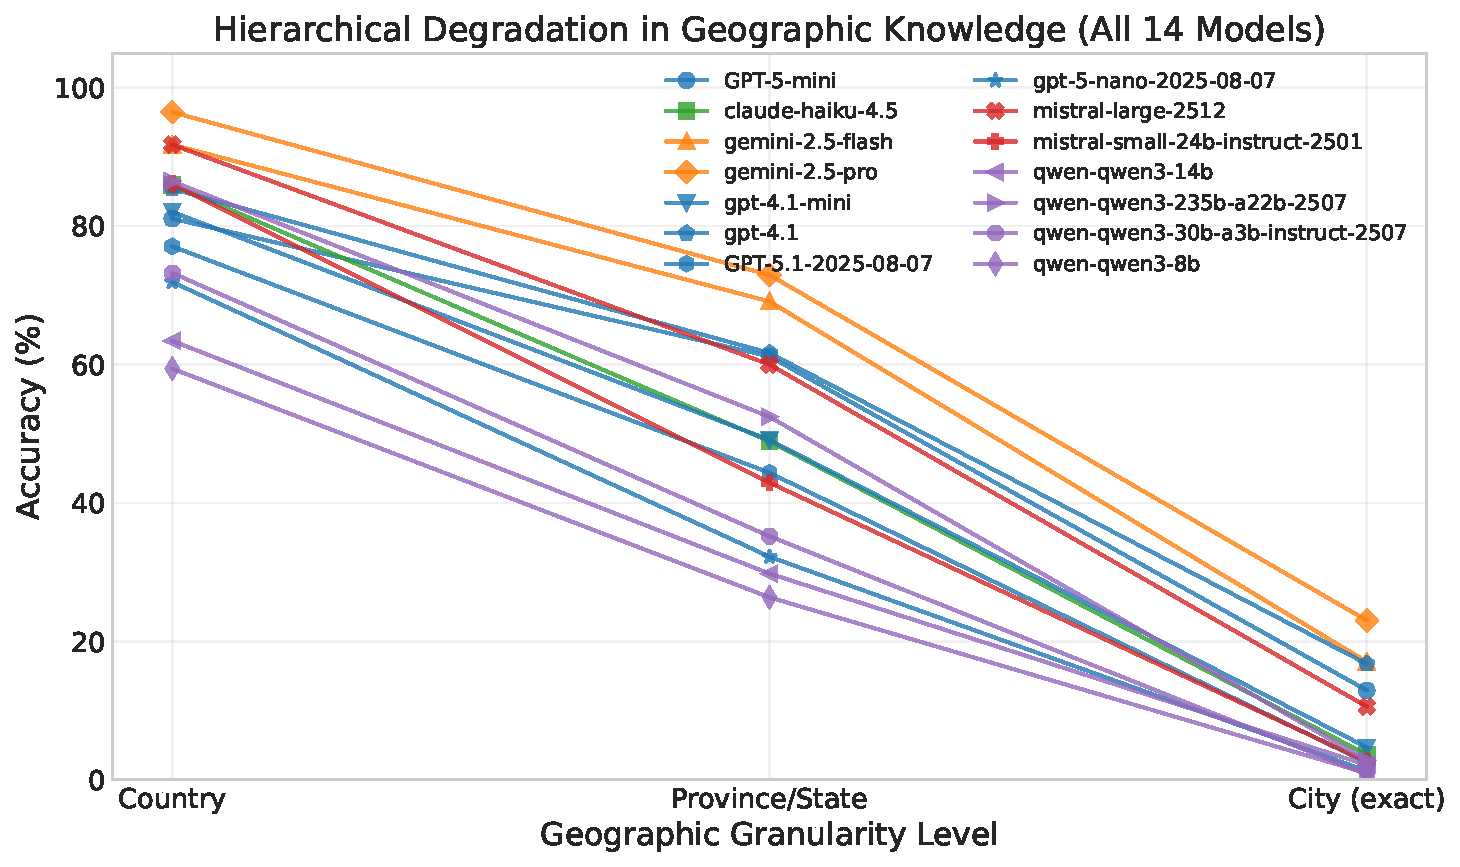
\includegraphics[width=\columnwidth]{figures/place_association_granularity_line.pdf}
\caption{Hierarchical degradation in geographic knowledge. Models perform well at country-level identification but accuracy drops sharply for finer granularities, with city-level accuracy below 25\% for all models.}
\label{fig:place_assoc_granularity}
\end{figure}

\begin{table}[htbp]
\centering
\caption{Place association accuracy (\%) by geographic granularity level. City requires exact match; other levels check if the correct name appears in the response.}
\label{tab:place_assoc_granularity}
\small
\begin{tabular}{lcccc}
\toprule
\textbf{Model} & \textbf{City} & \textbf{Province} & \textbf{Country} & \textbf{Region} \\
\midrule
Gemini-2.5-Pro & 23.0 & 72.9 & 96.5 & 40.0 \\
Gemini-2.5-Flash & 17.1 & 69.1 & 91.8 & 13.0 \\
GPT-4.1 & 16.8 & 61.7 & 85.4 & 1.4 \\
GPT-5.1 & 12.9 & 61.2 & 81.1 & 0.4 \\
Mistral-Large & 10.6 & 60.0 & 91.8 & 1.0 \\
GPT-4.1-mini & 4.7 & 49.1 & 82.1 & 2.4 \\
Claude-Haiku-4.5 & 3.6 & 48.9 & 86.0 & 38.4 \\
Qwen3-235B & 2.8 & 52.5 & 86.5 & 2.8 \\
Mistral-Small-24B & 2.6 & 42.9 & 86.1 & 7.0 \\
GPT-5-mini & 2.5 & 44.4 & 77.1 & 0.3 \\
GPT-5-nano & 1.3 & 32.2 & 71.9 & 0.2 \\
Qwen3-30B & 0.8 & 35.2 & 73.2 & 3.5 \\
\bottomrule
\end{tabular}
\end{table}

\paragraph{Finding.}
As illustrated in Figure~\ref{fig:place_assoc_granularity}, models exhibit a clear hierarchical degradation in geographic knowledge. Country-level identification is relatively strong (72--97\%), indicating models can generally locate coordinates within the correct nation. Province/state recognition drops to 32--73\%, showing partial knowledge of administrative divisions. However, exact city identification collapses to 1--23\%, revealing that models lack the fine-grained coordinate-to-city mappings required for precise reverse geocoding. This hierarchy suggests that LLMs encode geographic knowledge at coarse spatial resolutions but fail to learn the dense, precise mappings needed for city-level localization.
